% Fig. M1 - Modelo de cascada retroalimentada
% Unified style with the existing figures
% Compile: pdflatex fig_m1_cascada.tex
\documentclass[border=8pt]{standalone}
\usepackage[utf8]{inputenc}
\usepackage[T1]{fontenc}
\usepackage{amsmath}
\usepackage{tikz}
\usetikzlibrary{arrows.meta, positioning, calc}

\begin{document}
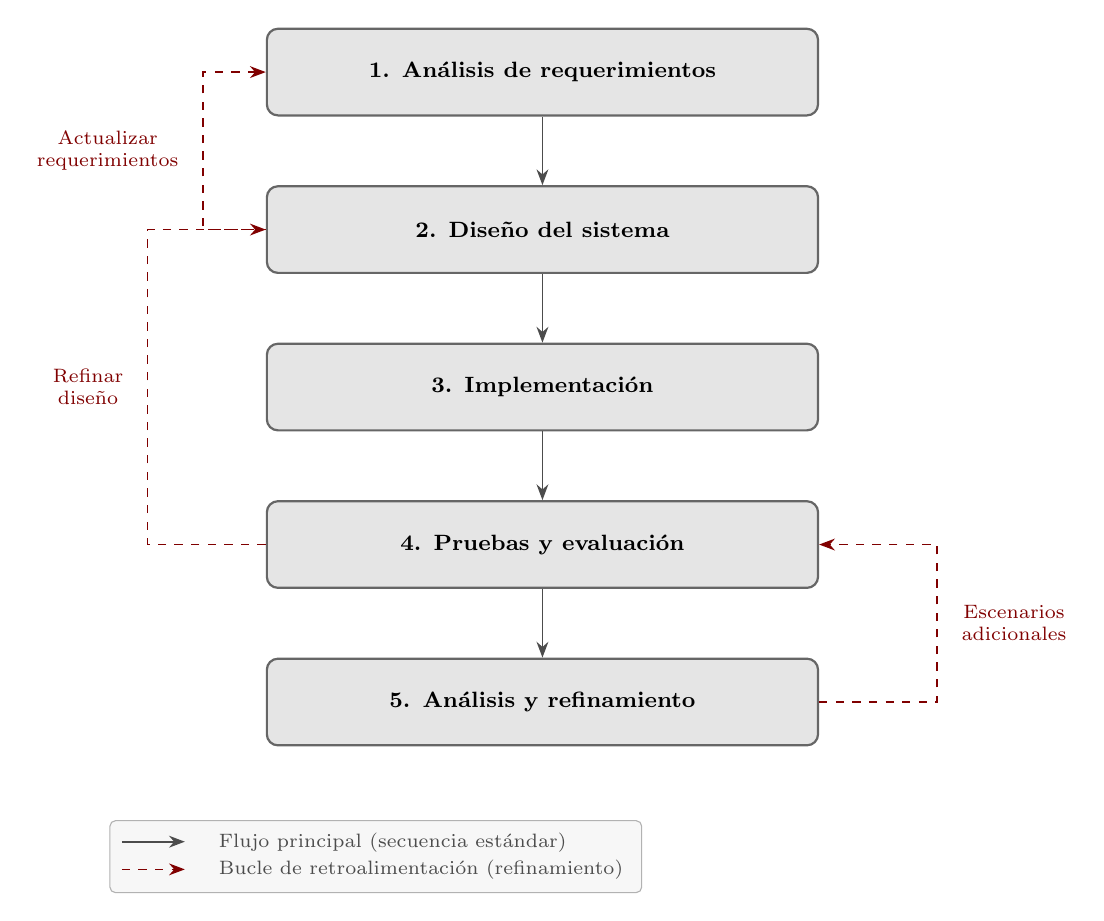
\begin{tikzpicture}[
    >=Stealth,
    font=\footnotesize,
    phase/.style={draw, rectangle, rounded corners=4pt,
                  minimum width=7cm, minimum height=1.1cm,
                  fill=black!5, thick, align=center,
                  font=\footnotesize\bfseries},
    current/.style={phase, fill=black!10, draw=black!60},
    flowarrow/.style={->, semithick, black!70},
    feedback/.style={->, semithick, red!50!black, dashed},
    fblabel/.style={font=\scriptsize, text=red!50!black, align=center},
    label/.style={font=\scriptsize, text=black!70, align=left},
]

% ============================================================
% PHASES (vertically stacked, explicit coordinates)
% ============================================================
\node[current] (f1) at (0,  0) {1. Análisis de requerimientos};
\node[current] (f2) at (0, -2) {2. Diseño del sistema};
\node[current] (f3) at (0, -4) {3. Implementación};
\node[current] (f4) at (0, -6) {4. Pruebas y evaluación};
\node[current] (f5) at (0, -8) {5. Análisis y refinamiento};

% ============================================================
% Main flow arrows (downward)
% ============================================================
\draw[flowarrow] (f1) -- (f2);
\draw[flowarrow] (f2) -- (f3);
\draw[flowarrow] (f3) -- (f4);
\draw[flowarrow] (f4) -- (f5);

% ============================================================
% Feedback arrows (straight, orthogonal routing — no curves)
% ============================================================

% (1) Pruebas (4) -> Diseño (2): left rail
\draw[feedback] (f4.west) -- ++(-1.5,0) |- (f2.west);
\node[fblabel, anchor=east] at (-5.2,-4) {Refinar\\diseño};

% (2) Diseño (2) -> Análisis de requerimientos (1): inner left rail
\draw[feedback] (f2.west) -- ++(-0.8,0) |- (f1.west);
\node[fblabel, anchor=east] at (-4.5,-1) {Actualizar\\requerimientos};

% (3) Análisis (5) -> Pruebas (4): right rail
\draw[feedback] (f5.east) -- ++(1.5,0) |- (f4.east);
\node[fblabel, anchor=west] at (5.2,-7) {Escenarios\\adicionales};

% ============================================================
% Legend
% ============================================================
\node[label, anchor=north west, draw=black!30, rounded corners=2pt,
      fill=black!3, inner sep=4pt] at (-5.5, -9.5) {
    \begin{tabular}{@{}l l@{}}
    \tikz[baseline=-2pt]{\draw[flowarrow] (0,0) -- (0.8,0);} & Flujo principal (secuencia estándar) \\[2pt]
    \tikz[baseline=-2pt]{\draw[feedback] (0,0) -- (0.8,0);} & Bucle de retroalimentación (refinamiento)
    \end{tabular}
};

\end{tikzpicture}
\end{document}
